%% =======================================================
%% Actividad 12: Ajuste de una distribución a datos reales
%%
%% Compilar desde actividades/: ./compilar.sh act12
%% Las figuras de img/ se generan con: python act12.py
%% =======================================================

%% ---- CONFIGURACIÓN ------------------------

\documentclass[11pt,letterpaper]{article}

\usepackage[indice]{tecnm}
\usepackage[T1]{fontenc}
\usepackage{amsmath}
\usepackage{xcolor}
\usepackage[most]{tcolorbox} % Carga tcolorbox con soporte para listings y saltos de página
\tcbuselibrary{listings, skins, breakable}
\setlength{\emergencystretch}{3em} % Evita líneas desbordadas por palabras en \texttt

% Paleta de colores (estilo GitHub Light / VS Code)
\definecolor{codebg}{HTML}{F8F9FA}       % Fondo del código
\definecolor{codehead}{HTML}{E9ECEF}     % Fondo de la barra de título
\definecolor{codeborder}{HTML}{CED4DA}   % Borde de la tarjeta
\definecolor{codetitle}{HTML}{212529}    % Texto del título
\definecolor{codekw}{HTML}{0550AE}       % Palabras clave (import, def, for...)
\definecolor{codefunc}{HTML}{8250DF}     % Funciones y métodos (describe, groupby...)
\definecolor{codestr}{HTML}{0A3069}      % Strings
\definecolor{codecomm}{HTML}{6E7781}     % Comentarios
\definecolor{codenum}{HTML}{8C959F}      % Números de línea
\definecolor{codeid}{HTML}{24292F}       % Texto general

% Configuración base de listings
\lstdefinestyle{pythonestilo}{
  language=Python,
  basicstyle=\ttfamily\footnotesize\color{codeid},
  keywordstyle=\color{codekw}\bfseries,
  keywordstyle=[2]\color{codefunc}, % Estilo secundario para métodos de datos
  stringstyle=\color{teal!80!black},
  commentstyle=\color{codecomm}\itshape,
  morekeywords={as, True, False, None, with, yield, lambda},
  morekeywords=[2]{print, len, sum, max, DataFrame, Series, value_counts, reindex, mean, std, var, randint, normal, seed, cumsum, poisson, binom, pmf, norm, fit, kde, bincount, linspace, train_test_split, make_blobs, GaussianNB, chisquare, pdf, cdf, hist, bar, plot, axhline, axvline, fill_between, subplots, figure, concat, nunique, load_iris, diff, sort, unique},
  numbers=left,
  numberstyle=\tiny\ttfamily\color{codenum},
  stepnumber=1,
  numbersep=10pt,
  showstringspaces=false,
  morestring=[b]{"""},
  tabsize=4,
  breaklines=true,
  breakatwhitespace=true,
  columns=flexible,
  keepspaces=true,
  literate=
    {á}{{\'a}}1 {é}{{\'e}}1 {í}{{\'i}}1 {ó}{{\'o}}1 {ú}{{\'u}}1
    {Á}{{\'A}}1 {É}{{\'E}}1 {Í}{{\'I}}1 {Ó}{{\'O}}1 {Ú}{{\'U}}1
    {ñ}{{\~n}}1 {Ñ}{{\~N}}1 {¿}{{?`}}1 {¡}{{!`}}1 {°}{{$^\circ$}}1
}

% Definición del entorno personalizado \begin{codigo}{Título}{etiqueta}
% \newtcblisting[auto counter, number within=section]{codigo}[2][]{
\newtcblisting[auto counter]{codigo}[2][]{
  listing only,
  breakable,                    % Permite que el bloque se divida si pasa de página
  enhanced,
  colback=codebg,
  colframe=codeborder,
  colbacktitle=codehead,
  coltitle=codetitle,
  fonttitle=\bfseries\small\sffamily,
  boxrule=0.6pt,
  arc=4pt,                      % Bordes redondeados
  left=20pt,                    % Espacio izquierdo para los números de línea
  right=8pt,
  top=6pt,
  bottom=6pt,
  toptitle=4pt,
  bottomtitle=4pt,
  before skip=12pt,
  after skip=12pt,
  listing options={style=pythonestilo},
  title={Código \thetcbcounter: #2},
  #1
}

% Paleta para salida de consola (estilo terminal limpia)
\definecolor{termbg}{HTML}{212529}      % Fondo oscuro tipo terminal
\definecolor{termhead}{HTML}{343A40}    % Barra superior
\definecolor{termtext}{HTML}{F8F9FA}    % Texto claro de alta legibilidad
\definecolor{termborder}{HTML}{495057}  % Borde

% Entorno \begin{consola}[label=out:iris]{Título}
\newtcblisting[auto counter]{consola}[2][]{
  listing only,
  breakable,
  colback=termbg,
  colframe=termborder,
  colbacktitle=termhead,
  coltitle=termtext,
  colupper=termtext,
  fonttitle=\bfseries\small\sffamily,
  boxrule=0.6pt,
  arc=4pt,
  left=8pt,
  right=8pt,
  top=6pt,
  bottom=6pt,
  toptitle=4pt,
  bottomtitle=4pt,
  before skip=12pt,
  after skip=12pt,
  listing options={
    basicstyle=\ttfamily\scriptsize\color{termtext}, % \scriptsize evita que las tablas de Pandas se partan de línea
    breaklines=true,
    columns=fixed,        % Mantiene alineadas las columnas de Pandas
    keepspaces=true,
    showstringspaces=false,
    literate=
      {á}{{\'a}}1 {é}{{\'e}}1 {í}{{\'i}}1 {ó}{{\'o}}1 {ú}{{\'u}}1
      {Á}{{\'A}}1 {É}{{\'E}}1 {Í}{{\'I}}1 {Ó}{{\'O}}1 {Ú}{{\'U}}1
      {ñ}{{\~n}}1 {Ñ}{{\~N}}1 {°}{{$^\circ$}}1
  },
  title={Salida \thetcbcounter: #2},
  #1
}

%% ---- DATOS DE LA MATERIA ------------------------

\materia{Modelos Estadísticos para el Aprendizaje \\ Automático y Ciencia de Datos}
\actividad{Tema 2.2
Distribuciones de Probabilidad Discretas y Continuas \\ Actividad 12 - Ajuste de una Distribución a Datos Reales}

\profesor{Dr. José Ismael Ojeda Campaña}
%\fecha{15 de octubre de 2026}    % opcional; por defecto es la fecha de hoy

\begin{document}
\portada
\indicegeneral

%% ---- CONTENIDO ---------------------------------

\section{Introducción}

Ajustar una distribución a datos reales consiste en elegir un modelo probabilístico, estimar sus parámetros a partir de la muestra y comprobar qué tan bien describe lo observado \parencite{tecnm2026_documento_fuente}. Es el paso que une la teoría de las distribuciones con los datos: en lugar de simular una distribución conocida, se parte de datos y se pregunta cuál modelo los explica mejor.

En este documento se ajustan distribuciones discretas y continuas al conjunto de datos del Titanic. Primero se estudia la edad de los pasajeros, con dos modelos discretos (Poisson y binomial) y tres continuos (normal, exponencial y gamma). Después se estudia un conteo, el número de hermanos o cónyuges a bordo, con modelos discretos (Poisson, binomial y geométrico) y continuos (normal y exponencial). En ambos casos se grafica el histograma con las curvas ajustadas, se evalúa el ajuste con el error cuadrático medio, la verosimilitud y comparaciones visuales, y se discute cuál modelo es el más apropiado y por qué.

\section{Marco conceptual}

\subsection{Distribuciones discretas y continuas}

Una distribución discreta asigna probabilidad a cada valor posible mediante una función de masa $p(k)$, y una continua la describe con una función de densidad $f(x)$, de modo que las probabilidades son áreas bajo la curva \parencite{tecnm2026_documento_fuente}. La Tabla~\ref{tab:resumen} resume las distribuciones usadas en esta actividad \parencite{tecnm2026_documento_fuente,rice2006}.

\begin{table}[htbp]
\centering
\caption{Distribuciones usadas en el ajuste.}
\label{tab:resumen}
\small
\renewcommand{\arraystretch}{1.6}
\begin{tabular}{llccc}
\hline
\textbf{Distribución} & \textbf{Masa o densidad} & \textbf{Media} & \textbf{Varianza} & \textbf{Parámetros} \\
\hline
Poisson$(\lambda)$ & $e^{-\lambda}\lambda^k/k!$ & $\lambda$ & $\lambda$ & 1 \\
Binomial$(n, p)$ & $\binom{n}{k}p^k(1-p)^{n-k}$ & $np$ & $np(1-p)$ & 1 ($n$ fijo) \\
Geométrica$(p)$ & $(1-p)^{k}p$, \; $k \ge 0$ & $(1-p)/p$ & $(1-p)/p^2$ & 1 \\
Normal$(\mu, \sigma)$ & $\dfrac{1}{\sigma\sqrt{2\pi}}e^{-(x-\mu)^2/(2\sigma^2)}$ & $\mu$ & $\sigma^2$ & 2 \\
Exponencial$(\lambda)$ & $\lambda e^{-\lambda x}$, \; $x \ge 0$ & $1/\lambda$ & $1/\lambda^2$ & 1 \\
Gamma$(\alpha, \lambda)$ & $\dfrac{\lambda^\alpha}{\Gamma(\alpha)}x^{\alpha-1}e^{-\lambda x}$ & $\alpha/\lambda$ & $\alpha/\lambda^2$ & 2 \\
\hline
\end{tabular}
\end{table}

La geométrica de la tabla cuenta los fracasos antes del primer éxito, de modo que empieza en $k = 0$. En el documento fuente se define como el número de ensayos hasta el primer éxito ($k \ge 1$), así que la versión usada aquí es la misma desplazada una unidad. Como en el documento fuente, en la exponencial y la gamma $\lambda$ es una tasa, y \texttt{scipy} recibe la escala $1/\lambda$.

\subsection{Estimación de parámetros por máxima verosimilitud}

Ajustar un modelo requiere estimar sus parámetros. El método de máxima verosimilitud elige los valores que hacen más probable la muestra observada. Para las distribuciones de esta actividad el resultado es sencillo: en la Poisson, $\hat\lambda$ es la media muestral; en la normal, $\hat\mu$ es la media y $\hat\sigma$ la desviación estándar con divisor $n$; en la exponencial, $1/\hat\lambda$ es la media; y en la geométrica, $\hat p = 1/(1 + \bar{x})$. En la binomial se fija $n$ en el valor máximo observado y se toma $\hat p = \bar{x}/n$. La gamma no tiene fórmula cerrada y \texttt{stats.gamma.fit()} la obtiene numéricamente.

\subsection{Cómo evaluar un ajuste}

El documento fuente propone comparar visualmente la distribución supuesta con los datos: el histograma con la curva de densidad superpuesta y el gráfico Q-Q, en el que los puntos deben caer sobre una recta si los datos siguen la distribución supuesta \parencite{tecnm2026_documento_fuente,bruce2020}. Para cuantificar el ajuste, el documento fuente menciona el error cuadrático medio (MSE) como métrica de evaluación \parencite{tecnm2026_documento_fuente}. Aquí se aplica a las proporciones: si $o_k$ es la proporción observada del valor $k$ y $p_k$ la que asigna el modelo,
\begin{equation}
\mathrm{MSE} = \frac{1}{m}\sum_{k}(o_k - p_k)^2 ,
\end{equation}
donde $m$ es el número de valores comparados.

Para comparar una masa discreta con una densidad continua hace falta una escala común, que es la probabilidad de cada valor entero. En un modelo discreto es $p(k)$, y en uno continuo es el área bajo la densidad en el intervalo que corresponde a $k$: $[k, k+1)$ para años cumplidos y $[k - 0.5, k + 0.5)$ para conteos (corrección por continuidad). Sobre esta misma escala se calcula además la log-verosimilitud $\ell$ de los datos agrupados y el criterio de Akaike, $\mathrm{AIC} = 2q - 2\ell$, donde $q$ es el número de parámetros estimados; un AIC menor indica mejor ajuste penalizando la complejidad. Estas dos medidas son una extensión de lo pedido. Por último, la prueba de Kolmogorov-Smirnov compara la función acumulada empírica con la del modelo continuo \parencite{tecnm2026_documento_fuente}.

\section{Descripción de la actividad}

\textbf{Objetivo:} Aplicar los conceptos de ajuste de distribuciones a un conjunto de datos reales para identificar cuál modelo probabilístico describe mejor la información observada \parencite{tecnm2026_documento_fuente}.

La actividad consta de cinco tareas:

\begin{description}
    \item[1) Selección de datos.] Elegir un conjunto de datos numéricos (propio o de acceso público).
    \item[2) Visualización inicial.] Graficar un histograma con curva de densidad.
    \item[3) Ajuste de modelo.] Probar al menos dos distribuciones (una discreta y una continua) para modelar los datos.
    \item[4) Evaluación.] Determinar cuál distribución se ajusta mejor con métricas como el error cuadrático medio o la comparación visual.
    \item[5) Conclusión.] Discutir los resultados y justificar la elección de la distribución más apropiada.
\end{description}

\section{Desarrollo}

Las tareas se resolvieron en el script \texttt{act12.py}, que usa \texttt{numpy}, \texttt{pandas}, \texttt{seaborn}, \texttt{scipy} y \texttt{matplotlib}. Las figuras se guardan como imágenes PNG en la carpeta \texttt{img/}. El Código~\ref{cod:comun} contiene las importaciones y la función auxiliar \texttt{guardar()}, que además muestra las figuras en pantalla cuando el código se ejecuta en un cuaderno. El cuaderno interactivo puede consultarse en Google Colab:

\begin{center}
    \url{https://colab.research.google.com/drive/1kITLYxO_-ATRKCMC2svGJTEeeSlcL_UD?usp=sharing}
\end{center}

\begin{codigo}[label=cod:comun]{Importaciones y función auxiliar}
import os

import matplotlib

# En Colab o Jupyter no existe __file__; ahí las figuras también se muestran en pantalla
EN_NOTEBOOK = '__file__' not in globals()
if not EN_NOTEBOOK:
    matplotlib.use('Agg')  # Como script, genera las figuras como archivos PNG sin abrir ventanas

import matplotlib.pyplot as plt
import numpy as np
import pandas as pd
import seaborn as sns
from scipy import stats

pd.set_option('display.width', 120)

# Carpeta donde se guardan las figuras que se incluyen en el reporte
BASE = os.getcwd() if EN_NOTEBOOK else os.path.dirname(os.path.abspath(__file__))
CARPETA_IMG = os.path.join(BASE, 'img')
os.makedirs(CARPETA_IMG, exist_ok=True)


def guardar(nombre):
    """Guarda la figura actual en la carpeta img/ y la muestra si se ejecuta en un notebook."""
    plt.tight_layout()
    plt.savefig(os.path.join(CARPETA_IMG, nombre), dpi=150)
    if EN_NOTEBOOK:
        plt.show()
    plt.close()
\end{codigo}

\subsection{Tarea 1: Selección de datos}

Se eligió el conjunto de datos del Titanic, de acceso público, que se carga con \texttt{sns.load\_dataset('titanic')} y contiene 891 pasajeros. Se modelaron dos variables numéricas (Código~\ref{cod:t1}). La primera es la edad, que falta en 177 pasajeros y por eso se analizan los 714 con edad registrada; se midió en años, pero la edad en años cumplidos (\texttt{np.floor}) es un conteo, y por eso se puede modelar tanto con distribuciones discretas como con continuas. La segunda es el número de hermanos o cónyuges a bordo (\texttt{sibsp}), un conteo genuino con los 891 pasajeros. Con dos variables de naturaleza distinta se puede ver si la mejor distribución cambia con los datos. La función \texttt{resumen()} calcula las medidas descriptivas, entre ellas el cociente varianza/media, que vale 1 en una Poisson.

\begin{codigo}[label=cod:t1]{Tarea 1: selección de datos}
# Conjunto de datos del Titanic (891 pasajeros).
# Variable 1: edad. Se mide en años (continua), pero la edad en años cumplidos es un
# conteo, así que se puede modelar con distribuciones discretas y continuas.
# Variable 2: número de hermanos o cónyuges a bordo (sibsp), un conteo.
titanic = sns.load_dataset('titanic')
edad = titanic['age'].dropna().to_numpy()   # 714 pasajeros con edad registrada
edad_cumplida = np.floor(edad).astype(int)  # años cumplidos
hermanos = titanic['sibsp'].to_numpy()      # 891 pasajeros


def resumen(x):
    """Medidas descriptivas; var/media cerca de 1 es lo esperado en una Poisson."""
    return pd.Series({
        'n': len(x), 'media': x.mean(), 'varianza': x.var(ddof=1),
        'var/media': x.var(ddof=1) / x.mean(), 'mínimo': x.min(), 'máximo': x.max(),
        'asimetría': stats.skew(x), 'curtosis': stats.kurtosis(x),
    })


print("=== Tarea 1: selección de datos (Titanic) ===")
print(f"Pasajeros: {len(titanic)}; con edad registrada: {len(edad)}; sin edad: {len(titanic) - len(edad)}")
print(pd.DataFrame({'edad (años cumplidos)': resumen(edad_cumplida),
                    'hermanos/cónyuges': resumen(hermanos)}).round(3).to_string())
\end{codigo}

\begin{consola}[label=out:out1]{Ejecución de \texttt{act12.py}: Tarea 1}
=== Tarea 1: selección de datos (Titanic) ===
Pasajeros: 891; con edad registrada: 714; sin edad: 177
           edad (años cumplidos)  hermanos/cónyuges
n                        714.000            891.000
media                     29.679              0.523
varianza                 211.309              1.216
var/media                  7.120              2.325
mínimo                     0.000              0.000
máximo                    80.000              8.000
asimetría                  0.383              3.689
curtosis                   0.173             17.774
\end{consola}

La edad tiene media 29.68 años, asimetría de 0.38 y un cociente varianza/media de 7.12: la varianza es siete veces mayor que la media, algo que una Poisson no admite. Los hermanos o cónyuges tienen media 0.52, varianza 1.22 (cociente 2.33), asimetría de 3.69 y un máximo de 8, es decir, una cola derecha larga.

\subsection{Tarea 2: Visualización inicial}

El Código~\ref{cod:t2} grafica el histograma de densidad de la edad con intervalos de 5 años y su curva de densidad estimada por kernel (KDE), que no supone ninguna forma, y las proporciones de los conteos de hermanos o cónyuges en un gráfico de barras (Figura~\ref{fig:inicial}).

\begin{codigo}[label=cod:t2]{Tarea 2: visualización inicial}
# Histograma con curva de densidad (KDE) de la edad y gráfico de barras de sibsp
fig, (ax1, ax2) = plt.subplots(1, 2, figsize=(13, 4.5))
x = np.linspace(0, 85, 400)
ax1.hist(edad, bins=np.arange(0, 85, 5), density=True, color='skyblue', edgecolor='black',
         alpha=0.7, label='Histograma (5 años)')
ax1.plot(x, stats.gaussian_kde(edad)(x), color='navy', linewidth=2, label='Curva de densidad (KDE)')
ax1.set_title('Edad de los pasajeros del Titanic')
ax1.set_xlabel('Edad (años)')
ax1.set_ylabel('Densidad')
ax1.legend()
ax1.grid(linestyle='--', alpha=0.5)

valores_h = np.arange(0, hermanos.max() + 1)
frec_h = np.array([(hermanos == k).mean() for k in valores_h])
ax2.bar(valores_h, frec_h, color='skyblue', edgecolor='black', alpha=0.7, label='Frecuencia relativa')
ax2.set_title('Hermanos o cónyuges a bordo')
ax2.set_xlabel('Número (k)')
ax2.set_ylabel('Proporción de pasajeros')
ax2.legend()
ax2.grid(linestyle='--', alpha=0.5)
guardar('visualizacion_inicial.png')
\end{codigo}

\begin{figure}[htbp]
\centering
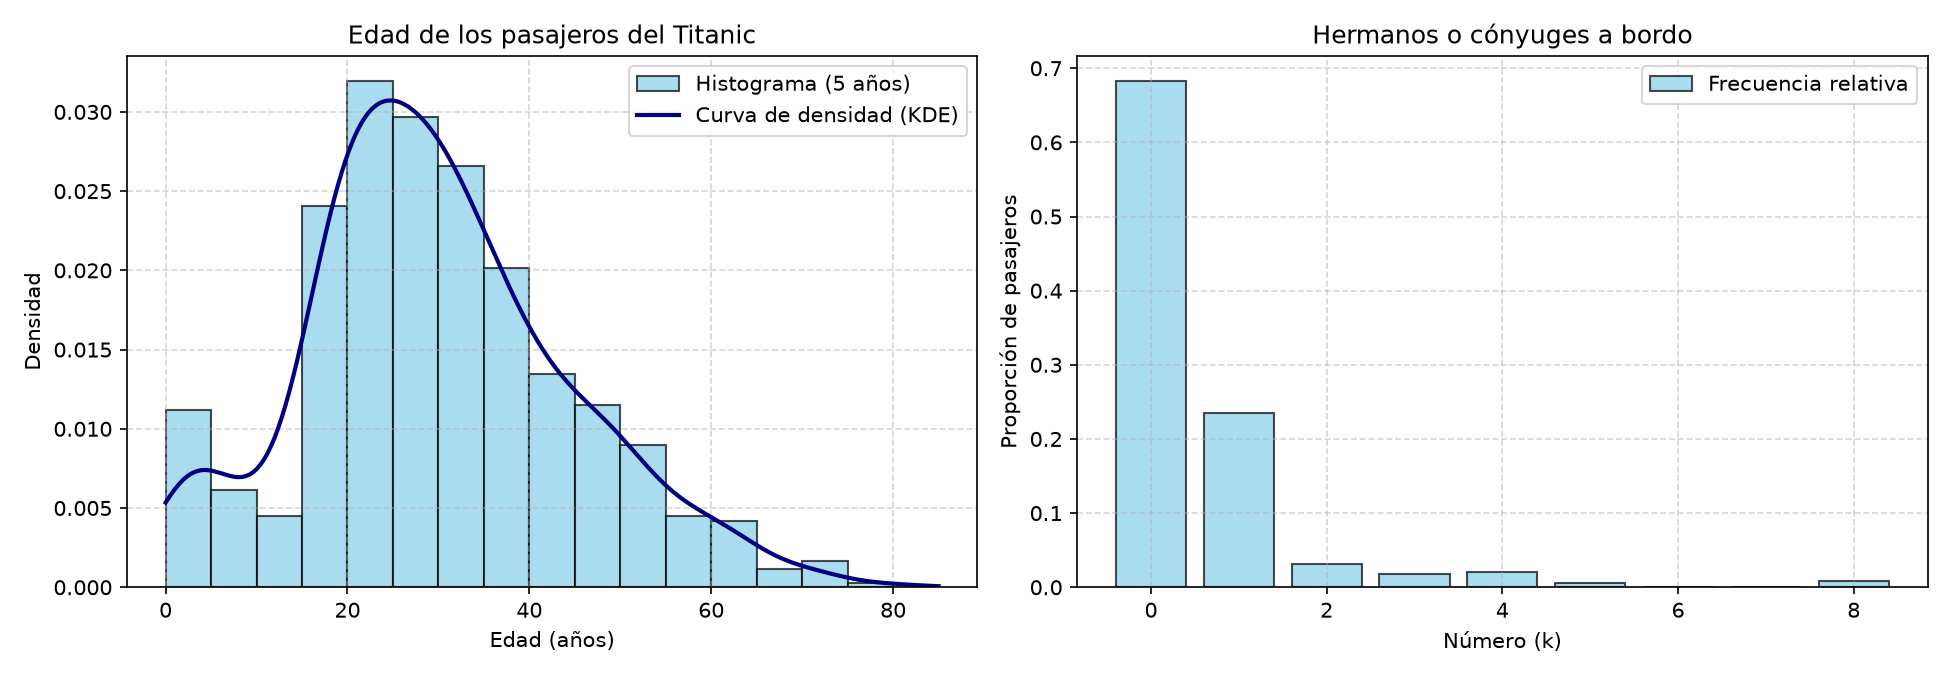
\includegraphics[width=\textwidth]{img/visualizacion_inicial.png}
\caption{Izquierda: histograma de la edad con su curva de densidad (KDE). Derecha: proporción de pasajeros según el número de hermanos o cónyuges a bordo.}
\label{fig:inicial}
\end{figure}

La edad tiene una moda cerca de los 20 a 30 años, una cola derecha que llega a los 80 y un pequeño grupo de niños menores de 5 años, que hace que la curva no sea del todo una campana. Los conteos de hermanos o cónyuges están concentrados en 0 (68\,\%) y 1 (23\,\%) y decrecen con rapidez, con una cola larga.

\subsection{Tarea 3: Ajuste de modelos}

El Código~\ref{cod:t3} ajusta los modelos con máxima verosimilitud. Para la edad se probaron dos distribuciones discretas (Poisson y binomial con $n = 80$, la edad máxima) y tres continuas (normal, exponencial y gamma). La función \texttt{probabilidades()} calcula la probabilidad de cada año según el modelo: la masa $p(k)$ si es discreto, o el área bajo la densidad en $[k, k+1)$ si es continuo. La Figura~\ref{fig:edad} muestra el histograma de años cumplidos, cuyas barras de un año miden directamente la proporción por año, con las curvas de los modelos.

\begin{codigo}[label=cod:t3]{Tarea 3: ajuste de modelos}
# Los parámetros se estiman por máxima verosimilitud. Las distribuciones del tema:
#   discretas: Poisson y binomial (y geométrica para los conteos)
#   continuas: normal, exponencial y gamma
# En la exponencial y la gamma, scipy usa la escala (1 / lambda del documento fuente).
def ajustar_edad():
    """Ajusta los cinco modelos a la edad. Devuelve {nombre: (distribución, tipo, parámetros)}."""
    media = edad_cumplida.mean()
    n_bin = int(edad_cumplida.max())                  # número de pruebas de la binomial
    mu, sigma = stats.norm.fit(edad)
    _, escala_exp = stats.expon.fit(edad, floc=0)     # escala = media
    alfa, _, escala_gam = stats.gamma.fit(edad, floc=0)
    return {
        'Poisson':     (stats.poisson(media), 'discreta', 1),
        'Binomial':    (stats.binom(n_bin, media / n_bin), 'discreta', 1),  # n fijo
        'Normal':      (stats.norm(mu, sigma), 'continua', 2),
        'Exponencial': (stats.expon(scale=escala_exp), 'continua', 1),
        'Gamma':       (stats.gamma(alfa, scale=escala_gam), 'continua', 2),
    }, dict(media=media, n_bin=n_bin, mu=mu, sigma=sigma, escala_exp=escala_exp,
            alfa=alfa, escala_gam=escala_gam)


def probabilidades(dist, tipo, valores, inicio):
    """Probabilidad que el modelo asigna a cada valor entero k.
    Discreta: pmf(k). Continua: área bajo la densidad en [k + inicio, k + inicio + 1)
    (inicio = 0 para años cumplidos; -0.5 para conteos, con corrección por continuidad)."""
    if tipo == 'discreta':
        return dist.pmf(valores)
    return dist.cdf(valores + inicio + 1) - dist.cdf(valores + inicio)


modelos_edad, par_edad = ajustar_edad()

print("\n=== Tarea 3: parámetros ajustados a la edad (máxima verosimilitud) ===")
print(f"Poisson:     lambda = {par_edad['media']:.3f}")
print(f"Binomial:    n = {par_edad['n_bin']}, p = {par_edad['media'] / par_edad['n_bin']:.4f}")
print(f"Normal:      mu = {par_edad['mu']:.3f}, sigma = {par_edad['sigma']:.3f}")
print(f"Exponencial: lambda = {1 / par_edad['escala_exp']:.4f}  (media 1/lambda = {par_edad['escala_exp']:.3f})")
print(f"Gamma:       alpha = {par_edad['alfa']:.3f}, lambda = {1 / par_edad['escala_gam']:.4f}")

# Histograma de años cumplidos con las curvas de los modelos. Con barras de 1 año, la
# altura del histograma es la proporción por año, comparable con pmf y densidad.
ks_edad = np.arange(0, 81)
obs_edad = np.array([(edad_cumplida == k).mean() for k in ks_edad])
colores = {'Poisson': 'tab:orange', 'Binomial': 'tab:green', 'Normal': 'tab:red',
           'Exponencial': 'tab:purple', 'Gamma': 'tab:blue'}

fig, (ax1, ax2) = plt.subplots(1, 2, figsize=(13, 4.5), sharey=True)
for ax, tipo in zip((ax1, ax2), ('continua', 'discreta')):
    ax.bar(ks_edad, obs_edad, width=1, align='edge', color='lightgray', edgecolor='gray',
           alpha=0.8, label='Observado (1 año)')
    for nombre, (dist, t, _) in modelos_edad.items():
        if t != tipo:
            continue
        p = probabilidades(dist, t, ks_edad, 0)
        estilo = '-' if t == 'continua' else 'o--'
        ax.plot(ks_edad + 0.5, p, estilo, color=colores[nombre], linewidth=2, markersize=3,
                label=nombre)
    ax.set_title(f'Modelos {tipo}s ajustados a la edad')
    ax.set_xlabel('Edad (años cumplidos)')
    ax.legend()
    ax.grid(linestyle='--', alpha=0.5)
ax1.set_ylabel('Probabilidad por año')
guardar('ajuste_edad.png')
\end{codigo}

\begin{consola}[label=out:out3]{Ejecución de \texttt{act12.py}: Tarea 3}
=== Tarea 3: parámetros ajustados a la edad (máxima verosimilitud) ===
Poisson:     lambda = 29.679
Binomial:    n = 80, p = 0.3710
Normal:      mu = 29.699, sigma = 14.516
Exponencial: lambda = 0.0337  (media 1/lambda = 29.699)
Gamma:       alpha = 2.715, lambda = 0.0914
\end{consola}

\begin{figure}[htbp]
\centering
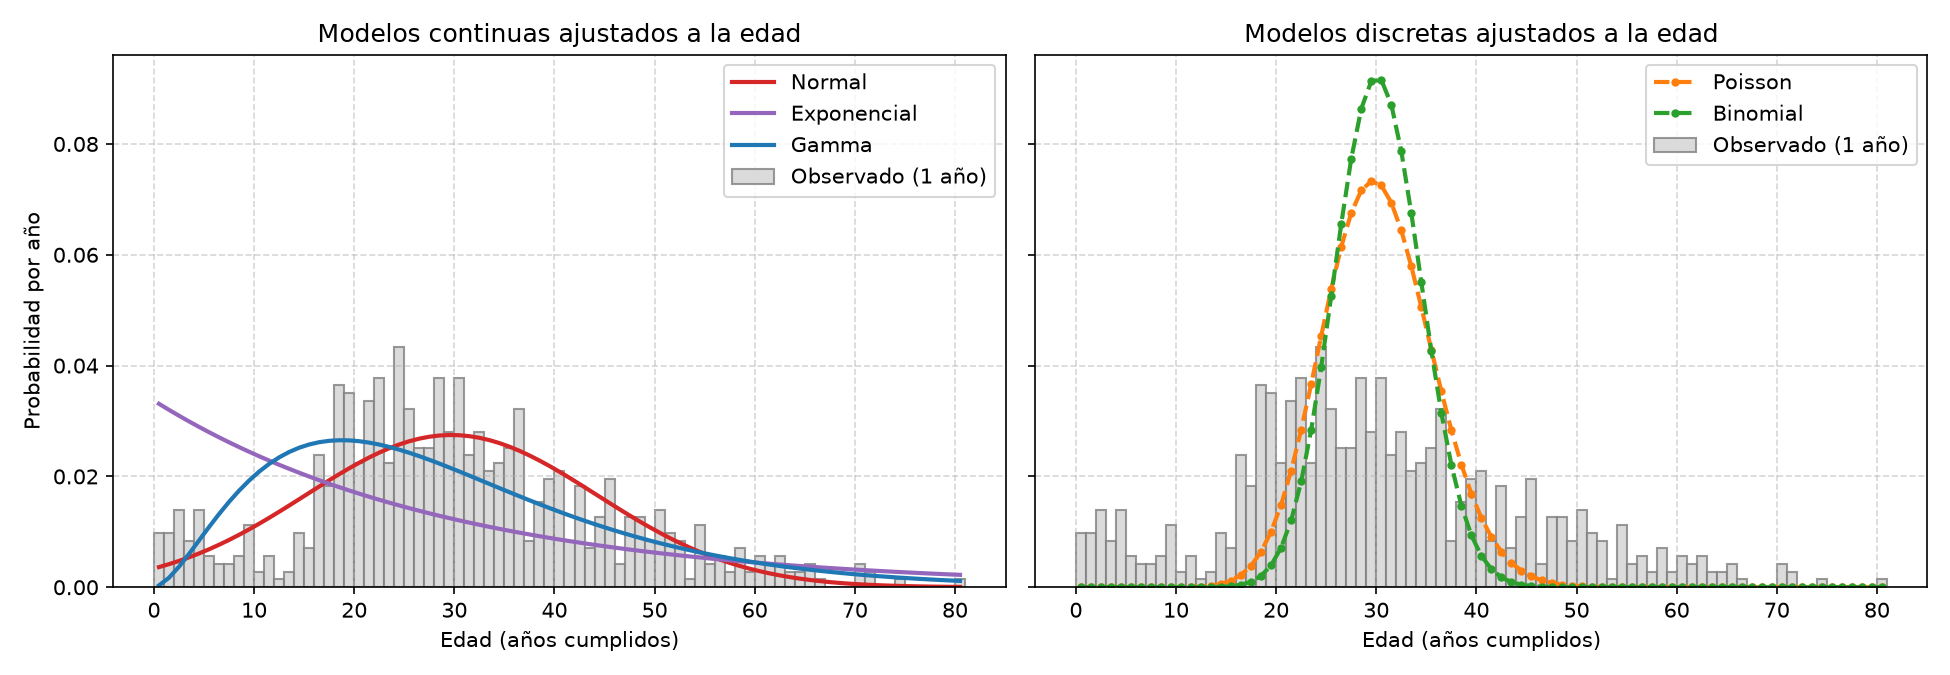
\includegraphics[width=\textwidth]{img/ajuste_edad.png}
\caption{Ajuste a la edad. Izquierda: modelos continuos. Derecha: modelos discretos. Las barras son la proporción observada por año cumplido.}
\label{fig:edad}
\end{figure}

Los modelos discretos no siguen la forma de los datos: la Poisson y la binomial producen una campana estrecha alrededor de 30 años, con una altura de 0.073 y 0.092 frente a cerca de 0.04 en los datos, y casi no asignan probabilidad a los menores de 15 años ni a los mayores de 45. La normal sigue la campana central y la gamma refleja la asimetría, mientras que la exponencial, que decrece desde 0, no concuerda con la moda de los datos.

\subsection{Tarea 4: Evaluación}

El Código~\ref{cod:t4} calcula el MSE, la raíz del MSE, el error máximo por año, la masa de probabilidad que cae en el rango observado, la log-verosimilitud y el AIC de cada modelo, y la prueba de Kolmogorov-Smirnov para los continuos. También grafica los gráficos Q-Q de la normal y la gamma y las funciones acumuladas (Figura~\ref{fig:qq}).

\begin{codigo}[label=cod:t4]{Tarea 4: evaluación}
def evaluar(modelos, valores, inicio, observado, n):
    """Error cuadrático medio entre las proporciones observadas y las del modelo, más
    verosimilitud y AIC sobre la misma escala (probabilidad de cada valor entero)."""
    filas = {}
    for nombre, (dist, tipo, k_par) in modelos.items():
        p = probabilidades(dist, tipo, valores, inicio)
        err = observado - p
        # Verosimilitud multinomial de los datos agrupados por valor
        loglik = float(np.sum(n * observado[observado > 0] * np.log(np.maximum(p[observado > 0], 1e-300))))
        filas[nombre] = {'tipo': tipo, 'MSE': np.mean(err ** 2), 'RMSE': np.sqrt(np.mean(err ** 2)),
                         'error máx.': np.abs(err).max(), 'masa en rango': p.sum(),
                         'logL': loglik, 'AIC': 2 * k_par - 2 * loglik}
    return pd.DataFrame(filas).T


tabla_edad = evaluar(modelos_edad, ks_edad, 0, obs_edad, len(edad_cumplida))
tabla_edad['MSE x 1e4'] = tabla_edad['MSE'].astype(float) * 1e4
print("\n=== Tarea 4: evaluación del ajuste a la edad (MSE sobre proporciones por año) ===")
print(tabla_edad[['tipo', 'MSE x 1e4', 'RMSE', 'error máx.', 'masa en rango', 'logL', 'AIC']]
      .sort_values('MSE x 1e4').astype({'MSE x 1e4': float, 'RMSE': float, 'error máx.': float,
                                        'masa en rango': float, 'logL': float, 'AIC': float})
      .round(4).to_string())

# Comparación visual adicional: Q-Q de los dos mejores continuos y función acumulada
fig, (ax1, ax2, ax3) = plt.subplots(1, 3, figsize=(14, 4.2))
probs = (np.arange(1, len(edad) + 1) - 0.5) / len(edad)
orden = np.sort(edad)
for ax, nombre in zip((ax1, ax2), ('Normal', 'Gamma')):
    teo = modelos_edad[nombre][0].ppf(probs)
    ax.plot(teo, orden, '.', color=colores[nombre], markersize=4)
    ax.plot([0, 80], [0, 80], 'k--', linewidth=1)
    ax.set_title(f'Gráfico Q-Q: {nombre}')
    ax.set_xlabel('Cuantiles del modelo')
    ax.set_ylabel('Cuantiles de la edad')
    ax.grid(linestyle='--', alpha=0.5)
ax3.step(orden, probs, color='black', linewidth=3, alpha=0.4, label='Empírica')
xs = np.linspace(0, 80, 400)
for nombre, (dist, tipo, _) in modelos_edad.items():
    cdf = dist.cdf(np.floor(xs)) if tipo == 'discreta' else dist.cdf(xs)
    ax3.plot(xs, cdf, color=colores[nombre], linewidth=1.5, label=nombre)
ax3.set_title('Función acumulada')
ax3.set_xlabel('Edad (años)')
ax3.legend(fontsize=8)
ax3.grid(linestyle='--', alpha=0.5)
guardar('qq_acumulada_edad.png')

# Prueba de Kolmogorov-Smirnov para los modelos continuos (edad sin redondear)
print("\nPrueba de Kolmogorov-Smirnov (modelos continuos, edad original):")
for nombre in ('Normal', 'Exponencial', 'Gamma'):
    ks = stats.kstest(edad, modelos_edad[nombre][0].cdf)
    print(f"  {nombre:<12} D = {ks.statistic:.4f}   p = {ks.pvalue:.4g}")
\end{codigo}

\begin{consola}[label=out:out4]{Ejecución de \texttt{act12.py}: Tarea 4}
=== Tarea 4: evaluación del ajuste a la edad (MSE sobre proporciones por año) ===
                 tipo  MSE x 1e4    RMSE  error máx.  masa en rango       logL         AIC
Normal       continua     0.3825  0.0062      0.0176         0.9794 -2924.1487   5852.2974
Gamma        continua     0.6521  0.0081      0.0220         0.9849 -2981.8125   5967.6251
Exponencial  continua     1.5624  0.0125      0.0287         0.9346 -3146.7675   6295.5350
Poisson      discreta     2.4408  0.0156      0.0456         1.0000 -4592.1609   9186.3217
Binomial     discreta     3.9263  0.0198      0.0633         1.0000 -6062.9515  12127.9030

Prueba de Kolmogorov-Smirnov (modelos continuos, edad original):
  Normal       D = 0.0646   p = 0.004963
  Exponencial  D = 0.3003   p = 1.37e-57
  Gamma        D = 0.1327   p = 2.032e-11
\end{consola}

\begin{figure}[htbp]
\centering
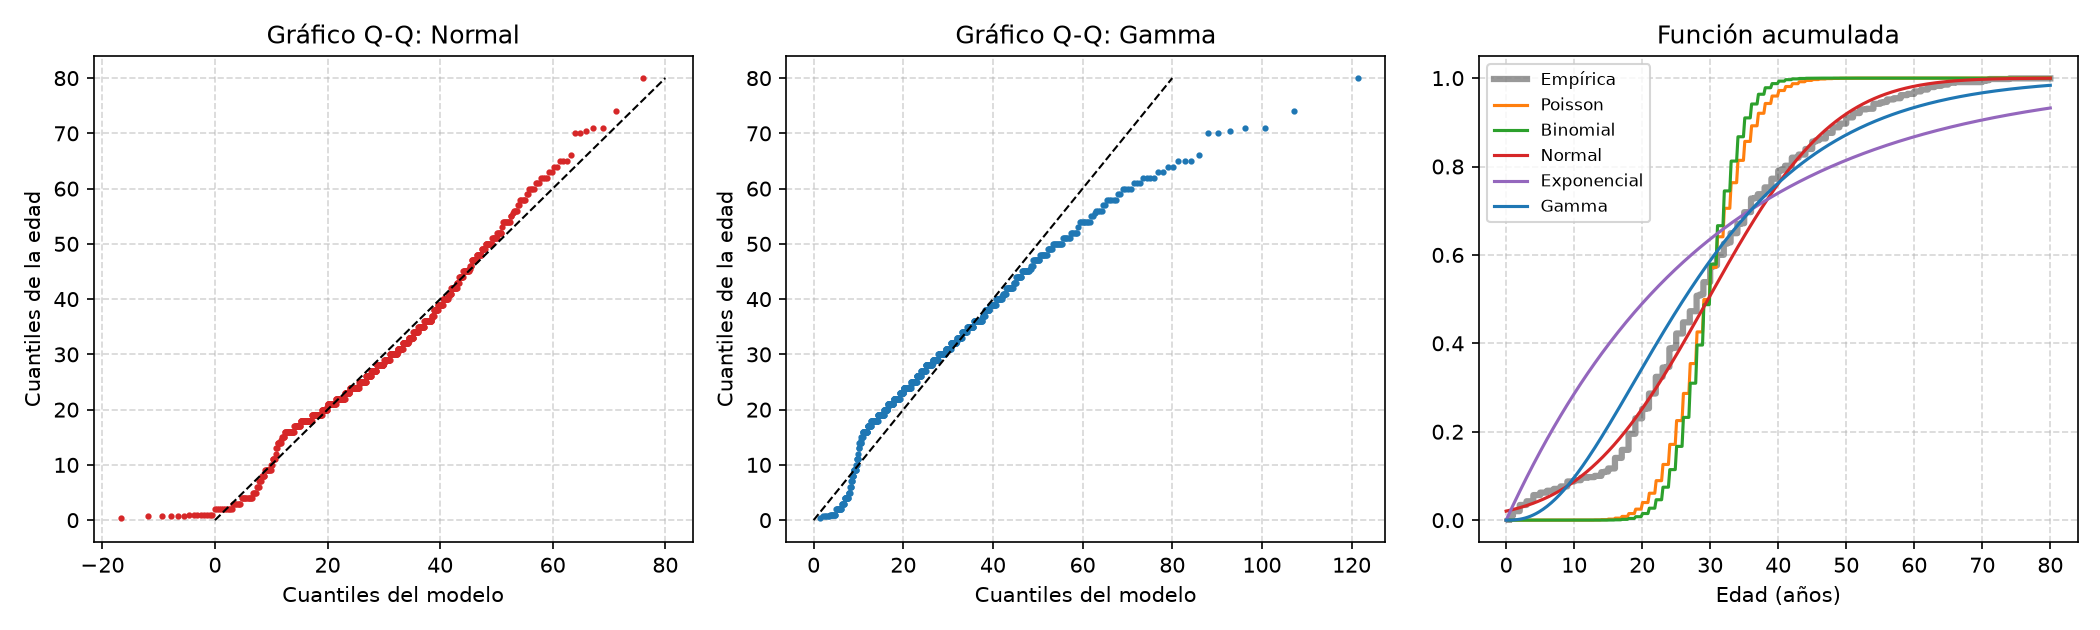
\includegraphics[width=\textwidth]{img/qq_acumulada_edad.png}
\caption{Edad: gráficos Q-Q de la normal y la gamma, y función acumulada empírica contra la de cada modelo.}
\label{fig:qq}
\end{figure}

\begin{table}[htbp]
\centering
\caption{Evaluación del ajuste a la edad, ordenada por MSE.}
\label{tab:edad}
\small
\begin{tabular}{llrrrr}
\hline
\textbf{Modelo} & \textbf{Tipo} & \textbf{MSE $\times 10^{4}$} & \textbf{Error máx.} & \textbf{AIC} & \textbf{Masa en rango} \\
\hline
Normal & continua & 0.383 & 0.018 & 5\,852 & 0.979 \\
Gamma & continua & 0.652 & 0.022 & 5\,968 & 0.985 \\
Exponencial & continua & 1.562 & 0.029 & 6\,296 & 0.935 \\
Poisson & discreta & 2.441 & 0.046 & 9\,186 & 1.000 \\
Binomial & discreta & 3.926 & 0.063 & 12\,128 & 1.000 \\
\hline
\end{tabular}
\end{table}

\begin{itemize}
    \item \textbf{Mejor modelo.} La normal tiene el menor MSE (0.383) y el menor AIC (5\,852), seguida de la gamma. Entre los discretos, la Poisson (MSE 2.44) es mejor que la binomial (3.93), pero ambos están muy por debajo de la normal y la gamma: su MSE es entre 6 y 10 veces mayor y su AIC es muy superior.
    \item \textbf{Por qué fallan los discretos.} La Poisson exige varianza igual a la media (29.7), pero la varianza observada es 211. La binomial, con $np(1-p) = 18.7$, tiene aún menos varianza que la media. Ninguna puede reproducir una dispersión tan grande, y por eso concentran la probabilidad en el centro.
    \item \textbf{Gráficos Q-Q.} En la normal los puntos siguen la recta en el centro, pero en la cola izquierda se separan: la normal asigna probabilidad a edades negativas (el cuantil más bajo del modelo es $-17$). Un 2\,\% de su masa queda fuera del rango $[0, 81)$. En la gamma ocurre lo contrario: sus cuantiles superiores son mayores que los datos (hasta 122 contra 80), es decir, su cola derecha es demasiado pesada.
    \item \textbf{Prueba de Kolmogorov-Smirnov.} Ningún modelo continuo es compatible con los datos al 5\,\%: la normal tiene $D = 0.065$ ($p = 0.005$), la gamma $D = 0.133$ y la exponencial $D = 0.300$. La normal es la mejor, pero la prueba detecta sus diferencias con los datos, entre ellas el grupo de niños.
\end{itemize}

\subsection{Segunda variable: hermanos o cónyuges a bordo}

Con los conteos de hermanos o cónyuges se repitió el procedimiento (Código~\ref{cod:t5}) con tres modelos discretos (Poisson, binomial con $n = 8$ y geométrico con $\hat p = 1/(1+\bar x) = 0.657$) y dos continuos (normal y exponencial con $\lambda = 1/\bar{x}$). Para los modelos continuos se usó la corrección por continuidad, con intervalos $[k - 0.5, k + 0.5)$.

\begin{codigo}[label=cod:t5]{Segunda variable: hermanos o cónyuges}
# Aquí los datos son conteos genuinos; se espera que un modelo discreto sea competitivo.
media_h = hermanos.mean()
modelos_h = {
    'Poisson':     (stats.poisson(media_h), 'discreta', 1),
    'Binomial':    (stats.binom(int(hermanos.max()), media_h / hermanos.max()), 'discreta', 1),
    # Geométrica con soporte 0, 1, 2, ...: P(k) = (1 - p)^k p, con p = 1 / (1 + media)
    'Geométrica':  (stats.geom(1 / (1 + media_h), loc=-1), 'discreta', 1),
    'Normal':      (stats.norm(media_h, hermanos.std()), 'continua', 2),
    'Exponencial': (stats.expon(scale=media_h), 'continua', 1),
}
obs_h = np.array([(hermanos == k).mean() for k in valores_h])
tabla_h = evaluar(modelos_h, valores_h, -0.5, obs_h, len(hermanos))
tabla_h['MSE x 1e4'] = tabla_h['MSE'].astype(float) * 1e4

print("\n=== Segunda variable: hermanos o cónyuges (k = 0..8) ===")
print(f"Geométrica: p = {1 / (1 + media_h):.4f}; Poisson: lambda = {media_h:.4f}")
prob_h = pd.DataFrame({'observada': obs_h}, index=valores_h)
for nombre, (dist, tipo, _) in modelos_h.items():
    prob_h[nombre] = probabilidades(dist, tipo, valores_h, -0.5)
print(prob_h.round(4).to_string())
print(tabla_h[['tipo', 'MSE x 1e4', 'RMSE', 'error máx.', 'masa en rango', 'logL', 'AIC']]
      .sort_values('MSE x 1e4').astype({'MSE x 1e4': float, 'RMSE': float, 'error máx.': float,
                                        'masa en rango': float, 'logL': float, 'AIC': float})
      .round(4).to_string())

fig, ax = plt.subplots(figsize=(8, 4.5))
ancho = 0.8 / (len(modelos_h) + 1)
ax.bar(valores_h - 0.4, obs_h, width=ancho, align='edge', color='lightgray', edgecolor='gray',
       label='Observado')
col_h = {'Poisson': 'tab:orange', 'Binomial': 'tab:green', 'Geométrica': 'tab:blue',
         'Normal': 'tab:red', 'Exponencial': 'tab:purple'}
for i, nombre in enumerate(modelos_h):
    ax.bar(valores_h - 0.4 + ancho * (i + 1), prob_h[nombre], width=ancho, align='edge',
           color=col_h[nombre], label=nombre)
ax.set_xlabel('Hermanos o cónyuges a bordo (k)')
ax.set_ylabel('Probabilidad')
ax.set_title('Ajuste a los conteos de hermanos o cónyuges')
ax.legend()
ax.grid(linestyle='--', alpha=0.5, axis='y')
guardar('ajuste_hermanos.png')
\end{codigo}

\begin{consola}[label=out:out5]{Ejecución de \texttt{act12.py}: segunda variable}
=== Segunda variable: hermanos o cónyuges (k = 0..8) ===
Geométrica: p = 0.6566; Poisson: lambda = 0.5230
   observada  Poisson  Binomial  Geométrica  Normal  Exponencial
0     0.6824   0.5927    0.5822      0.6566  0.3150       0.6156
1     0.2346   0.3100    0.3258      0.2255  0.3206       0.3276
2     0.0314   0.0811    0.0798      0.0774  0.1513       0.0484
3     0.0180   0.0141    0.0112      0.0266  0.0330       0.0072
4     0.0202   0.0018    0.0010      0.0091  0.0033       0.0011
5     0.0056   0.0002    0.0001      0.0031  0.0002       0.0002
6     0.0000   0.0000    0.0000      0.0011  0.0000       0.0000
7     0.0000   0.0000    0.0000      0.0004  0.0000       0.0000
8     0.0079   0.0000    0.0000      0.0001  0.0000       0.0000
                 tipo  MSE x 1e4    RMSE  error máx.  masa en rango       logL        AIC
Geométrica   discreta     3.4757  0.0186      0.0460         0.9999  -872.9146  1747.8291
Exponencial  continua    15.5372  0.0394      0.0930         1.0000  -960.7048  1923.4097
Poisson      discreta    18.4820  0.0430      0.0896         1.0000  -971.4929  1944.9858
Binomial     discreta    23.5559  0.0485      0.1001         1.0000 -1032.5756  2067.1512
Normal       continua   174.8023  0.1322      0.3674         0.8234 -1354.1374  2712.2747
\end{consola}

\begin{figure}[htbp]
\centering
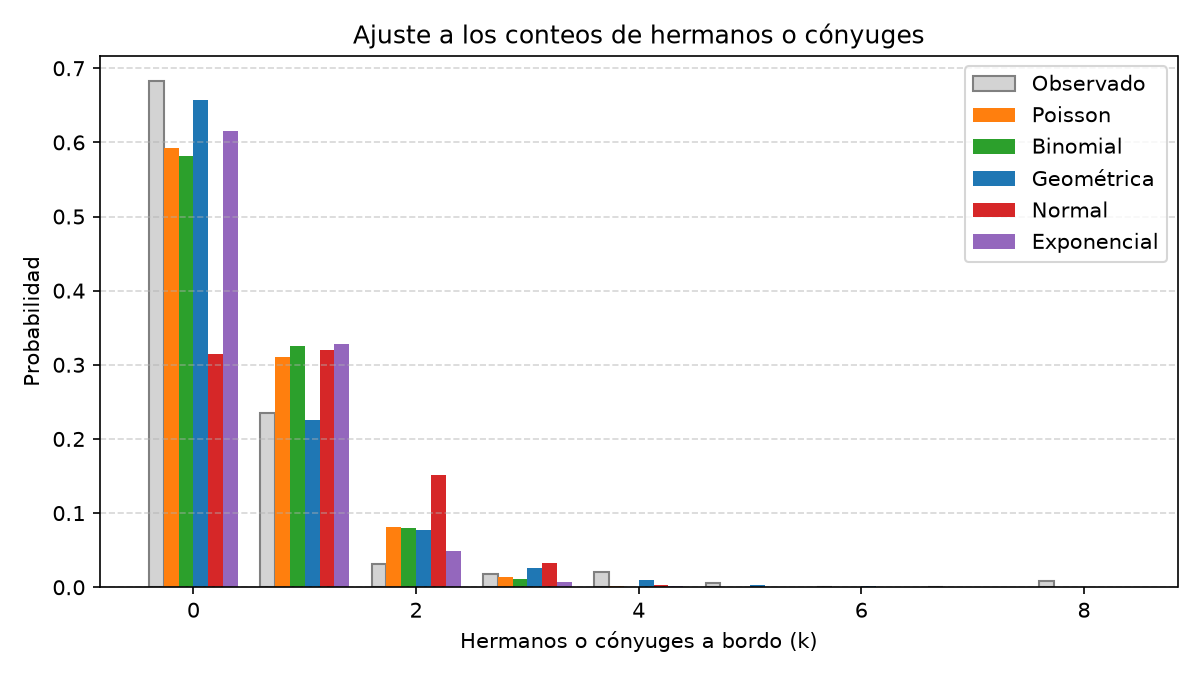
\includegraphics[width=0.8\textwidth]{img/ajuste_hermanos.png}
\caption{Probabilidad de cada número de hermanos o cónyuges: proporción observada y la asignada por cada modelo.}
\label{fig:hermanos}
\end{figure}

\begin{table}[htbp]
\centering
\caption{Evaluación del ajuste a los hermanos o cónyuges, ordenada por MSE.}
\label{tab:hermanos}
\small
\begin{tabular}{llrrrr}
\hline
\textbf{Modelo} & \textbf{Tipo} & \textbf{MSE $\times 10^{4}$} & \textbf{Error máx.} & \textbf{AIC} & \textbf{Masa en rango} \\
\hline
Geométrica & discreta & 3.48 & 0.046 & 1\,748 & 1.000 \\
Exponencial & continua & 15.54 & 0.093 & 1\,923 & 1.000 \\
Poisson & discreta & 18.48 & 0.090 & 1\,945 & 1.000 \\
Binomial & discreta & 23.56 & 0.100 & 2\,067 & 1.000 \\
Normal & continua & 174.80 & 0.367 & 2\,712 & 0.823 \\
\hline
\end{tabular}
\end{table}

\begin{itemize}
    \item \textbf{Mejor modelo.} La geométrica gana con el menor MSE (3.48, más de cuatro veces menor que el de la exponencial) y el menor AIC (1\,748). Reproduce bien el 0 (0.657 contra 0.682 observado) y el 1 (0.226 contra 0.235), y es la que asigna más probabilidad a las colas (0.0091 en $k = 4$, contra 0.0202 observado y 0.0018 de la Poisson).
    \item \textbf{Poisson y binomial.} Sobreestiman el 1 (0.31 y 0.33 contra 0.23) y subestiman el 0 y las colas. Su varianza (0.52 y 0.49) es menor que la observada (1.22); la de la geométrica, $(1-p)/p^2 = 0.80$, se acerca más.
    \item \textbf{Normal.} Es la peor (MSE 174.8): el 82\,\% de su masa cae en el rango observado, su moda queda en 1 y no puede producir una concentración del 68\,\% en 0 con cola larga.
    \item \textbf{Exponencial.} Es la mejor de las continuas, y su cercanía con la geométrica no es casual: con intervalos $[k, k+1)$ la exponencial discretizada es exactamente una geométrica. Con los intervalos centrados usados aquí solo se parece (por ejemplo, $P(0) = 0.616$ contra 0.657 de la geométrica).
\end{itemize}

\section{Conclusiones}

En la edad de los pasajeros, la mejor distribución fue la normal: tuvo el menor MSE (0.383 $\times 10^{-4}$) y el menor AIC, y la comparación visual lo confirma. La gamma quedó en segundo lugar y los modelos discretos fueron los peores, con MSE entre 6 y 10 veces mayor. La razón es la dispersión: la edad tiene una varianza siete veces mayor que su media y la Poisson y la binomial no permiten esa libertad. Hay que decir que la normal es solo la mejor de las opciones probadas y no un buen modelo en sentido estricto, porque la prueba de Kolmogorov-Smirnov la rechaza ($p = 0.005$): asigna un 2\,\% de probabilidad a edades fuera del rango y no recoge el grupo de niños pequeños.

En los hermanos o cónyuges ocurrió lo contrario: ganó un modelo discreto, la geométrica, con un MSE más de cuatro veces menor que el de la mejor continua y el menor AIC; la normal fue la peor. Se trata de un conteo con muchos ceros y una cola larga, que la geométrica, de un solo parámetro, representa bien, y que la Poisson no logra por tener varianza igual a la media.

La conclusión general es que la elección de la distribución depende de la naturaleza de la variable y de su dispersión, no de que sea discreta o continua en sí: una variable medida en años se ajusta mejor a una continua, y un conteo con sobredispersión a una geométrica. Un MSE bajo no basta por sí solo: conviene revisarlo junto con la comparación visual, la masa que el modelo pierde fuera del rango y una prueba formal como la de Kolmogorov-Smirnov.

\referencias

\end{document}
